% @Author: Yinlong Su
% @Date:   2015-10-30 16:15:47
% @Last Modified by:   Yinlong Su
% @Last Modified time: 2015-11-02 16:54:57

\documentclass[11pt]{article}
\usepackage{pgf-umlcd}
\usepackage[margin=.7in]{geometry}
\usepackage{wrapfig}
\usepackage{graphicx}
\usepackage{listings}
\usepackage{hyperref}
\usepackage[all]{hypcap}
\usepackage{tikz-er2}
\usetikzlibrary{shadows,positioning}
\usetikzlibrary{decorations, decorations.text,backgrounds}
\tikzset{every entity/.style={top color=white,bottom color=blue!30,draw=blue!50!black!100,drop shadow},
        every attribute/.style = {top color=white, bottom color=yellow!20,
                                  draw=yellow, drop shadow},
        every relationship/.style ={top color=white, bottom color=red!20,
                                  draw=red!50!black!100, drop shadow},
        every edge/.style = {link},
        every isa/.style = {top color=white, bottom color=green!20,
                                  draw=green!50!black!100, drop shadow},
        }


\begin{document}
\title{CSE532 Project Report\\\large Credit Card Database\\via the Object-Oriented Extension of SQL}
\author{Author Name, \#SBU ID}
\maketitle

\section{Database Design}
Something about design, general

\subsection{Entity-Relationship Design}
After a series of consideration, we decided the final Entity-Relationship Model as Figure \ref{fig:erccdb}.
\begin{figure}[!htp]
\centering

\begin{tikzpicture}[scale=0.8]

\node[entity] [draw] at (0, 0) (account) {Account};
\node[attribute] (number) [above = of account] {\key{Number}} edge (account);
\node[attribute] (balance) [above right = of account] {Balance} edge (account);
\node[attribute] (limit) [left = of account] {Limit} edge (account);

\node[isa] (isa1) [draw] at (0, -2) {IsA} edge (account);

\node[entity] (orgaccount) [draw] at (-2, -4) {OrgAccount} edge node [left] {disjoint} (isa1);
\node[entity] (peraccount) [draw] at (2, -4) {PerAccount} edge node [right] {covering} (isa1);

\node[relationship] (owns1) [draw] at (-2, -7) {Owns} edge [<-, very thick] (orgaccount);
\node[relationship] (owns2) [draw] at (2, -7) {Owns} edge [<-, very thick] (peraccount);

\node[entity] (organization) [draw] at (-2, -10) {Organization} edge (owns1);
\node[attribute] (id) [left = of organization] {\key{Id}} edge (organization);
\node[attribute] (name) [below left = of organization] {Name} edge (organization);
\node[attribute] (address) [below = of organization] {Address} edge (organization);

\node[entity] (person) [draw] at (4, -10) {Person} edge (owns2);
\node[attribute] (id) [above right = of person] {\key{Id}} edge (person);
\node[attribute] (name) [right = of person] {Name} edge (person);
\node[attribute] (address) [below right = of person] {Address} edge (person);
\node[attribute] (dob) [below = of person] {DOB} edge (person);

\node[relationship] (signs) [draw] at (1, -10) {Signs} edge (organization) edge (person);

\node [relationship] (authorizes) [draw] at (4, 0) {Authorizes} edge (account) edge(person);

\end{tikzpicture}
\caption{E-R diagram for CCDB}
\label{fig:erccdb}
\end{figure}

\subsubsection{Brief explanation of E-R design}
\label{sec:E-R design}

\par
Since the owner of a credit card account can be either a person or an organization, we split the accounts into two types: Personal Account and Organizational Account. This partition on Account satifies the disjointness constraint and covering constraint.

\par
After splitting the Account entity type into PerAccount and OrgAccount, we also split the relationship ``Owns''. But we don't need extra table to store these relationships. In fact, every account can have just one owner, no more and no less. We draw an arrow pointing in the direction of the relationship's diamond in very thick lines. We know that account Number is a key of PerAccount and also of PersonOwns. Thus, we can merge the attributes of PersonOwns into PerAccount. It is guaranteed that each PerAccount tuple has exactly one corresponding PersonOwns tuple, so no redundancy is created. Then we can concatenate PerAccount and PersonOwns tuples which have same account number, and the same goes to OrgAccount and OrganizationOwns.

\par
The relationship Signs and Authorizes are many-to-many relationships. We have to create tables to store the relation, and define proper foreign keys.

\subsubsection{Relational Database Schemas}
\par
Now we can convert the E-R diagram to relational database schemas. Noting that here we assume there is no inheritance and other object-oriented features. We keep Person and Organization entities. For account type hierarchy, we represent the IsA relationship in general representation. That means we create Account table stroing all information except owner. And table PerAccount and OrgAccount both have a foreign key pointing to Account and another foreign key pointing to the corresponding owner. The relationship Owns has been merged into PerAccount and OrgAccount. The SQL CREATE statements are as follows.
\begin{verbatim}
CREATE TABLE Person (
    Id      CHAR(20),
    Name    CHAR(20),
    Address CHAR(50),
    Dob     DATE,
    PRIMARY KEY (Id) )

CREATE TABLE Organization (
    Id      CHAR(20),
    Name    CHAR(20),
    Address CHAR(50)
    PRIMARY KEY (Id) )

CREATE TABLE Account (
    Number  CHAR(20),
    Balance DECIMAL,
    Limit   DECIMAL,
    PRIMARY KEY (Number) )

CREATE TABLE PerAccount (
    Number  CHAR(20),
    Owner   CHAR(20) NOT NULL,
    PRIMARY KEY (Number),
    FOREIGN KEY (Number) REFERENCES Account(Number),
    FOREIGN KEY (Owner) REFERENCES Person(Id) )

CREATE TABLE OrgAccount (
    Number  CHAR(20),
    Owner   CHAR(20) NOT NULL,
    PRIMARY KEY (Number),
    FOREIGN KEY (Number) REFERENCES Account(Number),
    FOREIGN KEY (Owner) REFERENCES Organization(Id) )

CREATE TABLE Signs (
    Pid CHAR(20),
    Oid CHAR(20),
    PRIMARY KEY (Pid, Oid),
    FOREIGN KEY (Pid) REFERENCES Person(Id),
    FOREIGN KEY (Oid) REFERENCES Organization(Id) )

CREATE TABLE Authorizes (
    Number CHAR(20),
    Pid    CHAR(20),
    PRIMARY KEY (Number, Pid),
    FOREIGN KEY (Number) REFERENCES Account(Number),
    FOREIGN KEY (Pid) REFERENCES Person(Id) )
\end{verbatim}

\subsection{Object-relational Design}

\par
The object-relational database concept provides us some very exciting features which will tremendously simplify the database schemas and query statements. Based on SQL 1999/2003 object extensions, we designed a draft schema of object-relational design of CCDB. The UML class diagram is shown as Figure \ref{fig:umlccdb}, and we also created the ODL-style schema.

\begin{verbatim}
interface Account: Object
    ( key: number )
{
    attribute string number;
    attribute numeric balance;
    attribute numeric limit;
    relationship Set<Person> authorizerdUsers inverse Person::authorizedAccounts;
}

class PerAccount: Account
{
    relationship Person owner inverse Person::accounts;
}

class OrgAccount: Account
{
    relationship Organization owner inverse Organization:accounts;
}

class Organization
    ( key: id )
{
    attribute string id;
    attribute string name;
    attribute string address;
    relationship SET<Account> accounts inverse OrgAccount::owner;
    relationship SET<Person> signers inverse Person::id;
}

class Person
    ( key: id )
{
    attribute string id;
    attribute string name;
    attribute string address;
    attribute date dob;
    relationship SET<Account> accounts inverse PerAccount::owner;
    relationship SET<Organization> signOrgs inverse Orgnization::id;
    relationship SET<Account> authorizedAccounts inverse Account::authorizedUsers;
}
\end{verbatim}

\begin{figure}[!htp]
\centering
\begin{tikzpicture}
    \begin{package}{Accounts}
        \begin{interface}[text width=7cm]{Account}{0,0}
            \attribute{number : string}
            \attribute{balance : numeric}
            \attribute{limit : numeric}
            \attribute{authorizedUsers : Person[]}
            \operation{getAuthorizedUsers : Person[]}
        \end{interface}

        \begin{class}[text width=5cm]{OrgAccount}{-5,-6}
            \attribute{owner : Organization}
            \implement{Account}
            \operation{getOwner() : Organzation}
        \end{class}

        \begin{class}[text width=5cm]{PerAccount}{5,-6}
            \attribute{owner : Person}
            \implement{Account}
            \operation{getOwner() : Person}
        \end{class}
    \end{package}
    \begin{class}[text width=5cm]{Organization}{-5,-9}
        \attribute{id : string}
        \attribute{name : string}
        \attribute{address : string}
        \attribute{accounts : Account[]}
        \attribute{signers : Person[]}
        \operation{getAccounts : Account[]}
        \operation{getSigners : Person[]}
    \end{class}
    \begin{class}[text width=6cm]{Person}{5,-9}
        \attribute{id : string}
        \attribute{name : string}
        \attribute{address: string}
        \attribute{dob : date}
        \attribute{accounts : Account[]}
        \attribute{signOrgs : Organization[]}
        \attribute{authorizedAccounts : Account[]}
        \operation{getAccounts() : Account[]}
        \operation{getSignableOrgs() : Organization[]}
        \operation{getAuthAccounts() : Account[]}
    \end{class}

    %\association{OrgAccount}{}{1..1}{Organization}{0..*}{}
    \draw [umlcd style] (OrgAccount) -- (Organization) node[near start, right]{1..1} node[near end, left]{0..*};
    %\association{PerAccount}{}{1..1}{Person}{0..*}{}
    \draw [umlcd style] (PerAccount) -- (Person) node[near start, right]{1..1} node[near end, left]{0..*};

    %\association{Organization}{0..*}{}{Person}{}{0..*}

    \draw [umlcd style] (Person.west |- 5, -12) -- (Organization.east |- -5, -12) node[near start, below]{0..*} node[near end, above]{0..*};

    \draw [umlcd style] (Account) -- (0,-11) node[near start, right]{0..*};
    \draw [umlcd style] (Person.west |- 5, -11) -- (0,-11) node[near start, above]{0..*};

\end{tikzpicture}
\caption{UML diagram for CCDB}
\label{fig:umlccdb}
\end{figure}

\par
With the power of object referencing, we can store all references into set-value types thus we do not need to create many relationship table/class. But unfortunately, PostgreSQL does not support all of the object-oriented features. In fact, it is very limited. Hence we have to adjust our design to cater to PostgreSQL.


\subsubsection{Account Type Hierarchy}

\par
We have briefly talked about the split of account type in section \ref{sec:E-R design}. Now we describe it in detail. The first problem we encountered is that the owner of a credit card account can be either a person or an organization. Although the sample test data has different ids between Person and Organization, we can not assume all data satifsies this condition. If we add a new enum column, which labeling the owner type, into Account, then we can distingish it by $(ownerId, ownerType)$. But then we have another problem: we can not define a proper foreign key constraint under ownerId column.

\begin{wrapfigure}{R}{0.5\textwidth}
\begin{tikzpicture}
    \begin{package}{Accounts}
        \begin{interface}[text width=3cm]{Account}{0,0}
            \attribute{...}
            \operation{...}
        \end{interface}

        \begin{class}[text width=3cm]{OrgAccount}{-2,-2}
            \attribute{...}
            \inherit{Account}
            \operation{...}
        \end{class}

        \begin{class}[text width=3cm]{PerAccount}{2,-2}
            \attribute{...}
            \inherit{Account}
            \operation{...}
        \end{class}
    \end{package}
\end{tikzpicture}
\caption{Hierarchy of Account Type}
\label{fig:accounthierarchy}
\end{wrapfigure}

\par
Therefore, we decided to split the accounts into two types: Personal Account and Organizational Account. All the attributes of Account type are applicable to subtype entities. We defined this IsA relationship that relates Account, PerAccount and OrgAccount. The role Sub refers to PerAccount and OrgAccount, while the role Super refers to Account. In the view of object-oriented, Account is a super class while PerAccount and OrgAccount are subclasses, as shown in Figure \ref{fig:accounthierarchy}. The subclasses inherit the features of the super class.
\par
In addition, our partition on Account is disjoint. A credit card account can not be a personal account and an organizational account at the same time. Thus we will not have duplicate tuples when inserting data into non-disjoint subtypes in PostgreSQL (we will discuss it later in section \label{ref:ptype}). And the partition also satisfies the covering constraint since the union of the sets of instances PerAccount and OrgAccount equals the set of instances of Account.
\par
We noticed that Person type and Organization type have many common attributes like id, name, address and they can both be the owner of a credit card account. A supertype, let us call it Owner, is not made for Person and Organization not only because we think those two types are essentially different but also they can not satisfy the covering constraint. If we create the Owner type for the convenience of defining the foreign key constraint of Account, then we can find some instances like `p2- John' in Person doesn't own any card.
\par


\subsubsection{Person Type Integrity}
\label{sec:ptype}

\begin{wrapfigure}{R}{0.5\textwidth}
\centering
\begin{tikzpicture}
    \begin{class}[text width=3cm]{Person}{0,0}
        \attribute{...}
        \operation{...}
    \end{class}

    \begin{class}[text width=3cm]{Signer}{-2,-2}
        \attribute{...}
        \inherit{Person}
        \operation{...}
    \end{class}

    \begin{class}[text width=3cm]{AuthorizedUser}{2,-2}
        \attribute{...}
        \inherit{Person}
        \operation{...}
    \end{class}
\end{tikzpicture}
\caption{Early partition on Person}
\label{fig:personhierarchy}
\end{wrapfigure}

\par
In our CCDB, a person can partcipate in many relationship. For example, a person can sign for an organization, can be authorized to use a card, and can also own some credit cards. Naturally, we can divide Person to Signer, AuthorizedUser and so on although the partition is not disjoint. At the begining we accept the Person Type Hierarchy and it seemed to have no big problem. But soon when we used PostgreSQL to insert data into tables, the trouble rose up.

\par
We used the concept of inheritance from object-oriented databases in PostgreSQL. Two tables, Signer and AuthorizedUser, inherit from Person. If we insert data into supertable Person, the subtables will have no data. That's understandable since the subtable has more attributes and constraints so that it can not extract data directly from supertable. But one person can be both a signer and an authorized user. If we insert data into subtables, we will have duplicate tuples in the view of supertable. For example `p4 - May' is a signer of organization `Acme', and also an authorized user of credit card c10. We insert the data of May into Signer and AuthorizedUser then we have two ``identical'' tuples in supertable Person.

\par
We quote ``identical'' because they are actually different tuples in PostgreSQL database. In PostgreSQL documents, the behavior is described as \emph{``INSERT always inserts into exactly the table specified."} Therefore, we have two different tuples with same values in table Signer and AuthorizedUser. When we run SELECT query on Person, PostgreSQL returns all data from tables inherited from Person.

\par
To show that, we modified the table to explicitly store OIDs. Then we ran the following SQL command and got the result as shown in Figure \ref{fig:qonperson}.
\begin{verbatim}
   SELECT oid, * FROM "Person";
\end{verbatim}

\begin{figure}[!htp]
\centering
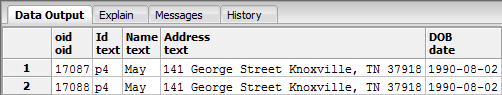
\includegraphics{F4.png}
\caption{Query on Person}
\label{fig:qonperson}
\end{figure}

\par
The tuples were not identical because they came from different tables and they had different OIDs. The same-value tuples did not violate the primary key constraint because table Person was empty. We can verify that by add ONLY keyword to the query and the query will return 0 result.
\begin{verbatim}
   SELECT oid, * FROM ONLY "Person";
\end{verbatim}

\par
In fact, that is not the only problem that inheritance of PostgreSQL rises. When we create a foreign key that points to a supertable, we will encounter exception saying that foreign key does not exist. It is because the supertable is usually empty and PostgreSQL does not extract data from subtables when handle foreign key constraints. This type of behavior has been described in the document:
\par
\emph{All check constraints and not-null constraints on a parent table are automatically inherited by its children. Other types of constraints (unique, primary key, and foreign key constraints) are not inherited.}
\par
As a result, we need to handle the foreign key constraints which point to a supertable very carefully. The best way is to avoid using that. But we can also create some triggers to ensure the data consistency. Based on the complexity of implementation and the performance on PostgreSQL, we decided not to partition the Person type.

\subsubsection{References in PostgreSQL}
\label{sec:refinpgsql}
\par
In SQL 1999/2003 object extensions, we can use object references to access related objects in a way similar to object-oriented language, like Java. In PostgreSQL, we can define a column type as an existing table. For example, we can define ``owner'' column as Person type in table PerAccount. But it is actually store a Person tuple in the column, not a real reference. PostgreSQL does not provide reference types. Instead, PostgreSQL has a kind of object identifier types. For safety issues, PostgreSQL only uses OIDs as primary keys for various system tables. User-created tables are not recommended to use OIDs.
\par
Using OIDs in our tables does not simplify the query in our system. No function or call is provided to convert OID to object. If we want to get the object the OID represents, we have to do join query. Basically, it has nothing different from using our own foreign keys.
\par
In addition, PostgreSQL does not support array element foreign key referencing. In our original object-relational design, we have some array attributes in our classes. PostgreSQL can not define foreign key references on array. At first we want to use CHECK constraint, but those CHECK constraints in PostgreSQL does not support nested query.
\par
So we have to use triggers to ensure the references if we want to use arrays in our tables. Or we can use extra relationship tables and foreign keys in an old way. It is ARRAY + TRIGGERS vs TABLE + FOREIGN KEY. We choose the latter in our final design and we have two reasons:
\par
\begin{enumerate}
\item Using so many triggers is inefficient. For every many-to-many relationship, if we use arrays, we have to create triggers on every foreign key constraint. The triggers are for the action taken after update and delete. If we want to ensure participation constraints, we have to create triggers before insert. We do not want to write so many triggers. Using build-in foreign key constraints of PostgreSQL is fine with us.
\item Space efficiencies are asymptotically equal. Stroing the reference ids in array or table takes exactly the same space. Even if we compare the space taken by managing array structure or by managing new table, those two ways have same space complexities.
\item Class methods are global in PostgreSQL. We define some methods that return required tuples in our original design before. PostgreSQL stores all functions under schema, not table. That means if we move the array references out of table into a new relationship table, all functions in PostgreSQL have same accessibility.
\end{enumerate}
\par
So we decide to use extra relationship tables and foreign key references to store all many-to-many relationships. We also have some methods under the schema to provide us some object-oriented features to simplify our query.
\par
There is another problem that our authorizes table needs to refer to Account table. We know that Account table actually has no tuples (we talked about this in section \ref{sec:ptype}). We need to create triggers for this particular foreign key constraint.

\subsubsection{CCDB Database on PostgreSQL}
\par
PostgreSQL has some object-relational database features. But many of them are different from what we think about. In this section we cretae our CCDB system on PostgreSQL. Before we go into details, we create a new UML class diagram for CCDB under PostgreSQL, as shown in Figure \ref{fig:newumlccdb}.
\par
We remove the package Account, and move owner attribute from OrgAccount and PerAccount to interface Account. The real foreign constraints will define in class OrgAccount and PerAccount. Also, we omit all 0..* labels on association lines. Finally, all functions are grouped in a yellow box, which indicates the schema function library.

\begin{figure}[!htp]
\centering
\renewcommand{\umldrawcolor}{black}
\renewcommand{\umlfillcolor}{blue!10}
\begin{tikzpicture}
    \begin{interface}[text width=4cm]{Account}{0,0}
        \attribute{number : text}
        \attribute{balance : numeric}
        \attribute{limit : numeric}
        \attribute{owner : text}
    \end{interface}

    \begin{class}[text width=2.5cm]{OrgAccount}{-5,-4}
        \implement{Account}
    \end{class}

    \begin{class}[text width=2.5cm]{PerAccount}{5,-4}
        \implement{Account}
    \end{class}
    \begin{class}[text width=5cm]{Organization}{-5,-7}
        \attribute{id : text}
        \attribute{name : text}
        \attribute{address : text}
    \end{class}
    \begin{class}[text width=5cm]{Person}{5,-7}
        \attribute{id : text}
        \attribute{name : text}
        \attribute{address: text}
        \attribute{dob : date}
    \end{class}

    \begin{class}[text width=5cm]{Signs}{-3,-10}
        \attribute{pid : text}
        \attribute{oid : text}
    \end{class}

    \begin{class}[text width=5cm]{Authorizes}{3,-10}
        \attribute{cid : text}
        \attribute{pid : text}
    \end{class}

    %\association{OrgAccount}{}{1..1}{Organization}{0..*}{}
    \draw [umlcd style] (OrgAccount) -- (Organization) node[near start, right]{1..1};
    %\association{PerAccount}{}{1..1}{Person}{0..*}{}
    \draw [umlcd style] (PerAccount) -- (Person) node[near start, right]{1..1};

    %\association{Organization}{0..*}{}{Person}{}{0..*}

    \draw [umlcd style] (Person.west |- 5, -9) -- (Organization.east |- -5, -9);

    \draw [umlcd style] (Account) -- (0,-8);
    \draw [umlcd style] (Person.west |- 5, -8) -- (0,-8);

    \draw [umlcd style dashed line] (-1, -9) -- (-1, -10);
    \draw [umlcd style dashed line] (1, -8) -- (1, -10);

    \node [draw, rectangle, align=left, fill=yellow!20] at (0, -15) {
 +getAuthorizedUsers(Account) : Person[] \\
 +getOOwner(Account) : Organzation \\
 +getPOwner(Account) : Person \\
 +getAccounts(Organization) : Account[] \\
 +getAccounts(Person) : Account[] \\
 +getSigners(Organization) : Person[] \\
 +getSignableOrgs(Person) : Organization[] \\
 +getAuthAccounts(Person) : Account[]};

\end{tikzpicture}
\caption{New UML diagram for CCDB}
\label{fig:newumlccdb}
\end{figure}


\paragraph{Using User-Defined Types in PostgreSQL}

\par
One of the important object-oriented features is user-defined types. PostgreSQL has UDTs but does not support the inheritance of UDTs. In our database, three UDTs are defined as accountType, organizationType and personType. The SQL commands are as follows:

\begin{verbatim}
CREATE TYPE public.accounttype AS
   ("number"  text,
    "balance" numeric,
    "limit"   numeric,
    "owner"   text);

CREATE TYPE public.organizationtype AS
   ("oid"     text,
    "name"    text,
    "address" text);

CREATE TYPE public.persontype AS
   ("pid"     text,
    "name"    text,
    "address" text,
    "dob"     date);
\end{verbatim}

\paragraph{Table Inheritance in PostgreSQL}
\par
PostgreSQL provides table inheritance. Based on the types and inheritance relationship, five tables are created as Account, OrgAccount, PerAccount, Organization and Person. We also create two relationship tables signs and authorizes. We include all primary key constraints and foreign key constraints as many as possible here.

\begin{verbatim}
CREATE TABLE public."Account"
OF accounttype
(
  "number" WITH OPTIONS  NOT NULL,
-- Inherited from type accounttype: "balance",
-- Inherited from type accounttype: "limit",
  "owner" WITH OPTIONS  NOT NULL,
  CONSTRAINT account_pkey PRIMARY KEY (number)
);

CREATE TABLE public."OrgAccount"
(
-- Inherited from table "Account":  "number" text NOT NULL,
-- Inherited from table "Account":  "balance" numeric,
-- Inherited from table "Account":  "limit" numeric,
-- Inherited from table "Account":  "owner" text NOT NULL,
  CONSTRAINT "OrgAccount_pkey" PRIMARY KEY (number),
  CONSTRAINT "OrgAccount_owner_fkey" FOREIGN KEY (owner)
      REFERENCES public."Organization" (oid) MATCH SIMPLE
      ON UPDATE CASCADE ON DELETE CASCADE
)
INHERITS (public."Account");

CREATE TABLE public."PerAccount"
(
-- Inherited from table "Account":  "number" text NOT NULL,
-- Inherited from table "Account":  "balance" numeric,
-- Inherited from table "Account":  "limit" numeric,
-- Inherited from table "Account":  "owner" text NOT NULL,
  CONSTRAINT "PerAccount_pkey" PRIMARY KEY (number),
  CONSTRAINT "PerAccount_owner_fkey" FOREIGN KEY (owner)
      REFERENCES public."Person" (pid) MATCH SIMPLE
      ON UPDATE CASCADE ON DELETE CASCADE
)
INHERITS (public."Account");

CREATE TABLE public."Organization"
OF organizationtype
(
  oid WITH OPTIONS  NOT NULL,
-- Inherited from type organizationtype: name,
-- Inherited from type organizationtype: address,
  CONSTRAINT organization_pkey PRIMARY KEY (oid)
);

CREATE TABLE public."Person"
OF persontype
(
  pid WITH OPTIONS  NOT NULL,
-- Inherited from type persontype: name,
-- Inherited from type persontype: address,
-- Inherited from type persontype: dob,
  CONSTRAINT person_pkey PRIMARY KEY (pid)
);

CREATE TABLE public.signs
(
  pid text NOT NULL,
  oid text NOT NULL,
  CONSTRAINT signs_pkey PRIMARY KEY (pid, oid),
  CONSTRAINT signs_oid_fkey FOREIGN KEY (oid)
      REFERENCES public."Organization" (oid) MATCH SIMPLE
      ON UPDATE CASCADE ON DELETE CASCADE,
  CONSTRAINT signs_pid_fkey FOREIGN KEY (pid)
      REFERENCES public."Person" (pid) MATCH SIMPLE
      ON UPDATE CASCADE ON DELETE CASCADE
);

CREATE TABLE public.authorizes
(
  cid text NOT NULL,
  pid text NOT NULL,
  CONSTRAINT authorizes_pkey PRIMARY KEY (cid, pid),
  CONSTRAINT authorizes_pid_fkey FOREIGN KEY (pid)
      REFERENCES public."Person" (pid) MATCH SIMPLE
      ON UPDATE CASCADE ON DELETE CASCADE
);
\end{verbatim}

\paragraph{Triggers}
\par
We talked about we need triggers to ensure the constraints pointing to a supertable in section \ref{sec:refinpgsql}. We create two triggers. One executes before insert or update on table authorizes. The other one executes after update or delete on Account. But since the real data is stored in OrgAccount and PerAccount, we should create triggers on OrgAccount and PerAccount.

\begin{verbatim}
CREATE OR REPLACE FUNCTION public.tf_iu_authorizes()
  RETURNS trigger AS
$BODY$
  BEGIN
    -- Check the insert/update row has correct account number in text array owns
    IF (NEW.cid IN (SELECT pa.number FROM "PerAccount" pa)) OR (NEW.cid IN (SELECT oa.number FROM "OrgAccount" oa)) THEN
      RETURN NEW;
    END IF;
    RAISE EXCEPTION '% is not a valid account number.', NEW.cid;
  END;
$BODY$
  LANGUAGE plpgsql;

CREATE TRIGGER tf_iu_authorizes
  BEFORE INSERT OR UPDATE
  ON public.authorizes
  FOR EACH ROW
  EXECUTE PROCEDURE public.tf_iu_authorizes();

CREATE OR REPLACE FUNCTION public.tf_ud_account()
  RETURNS trigger AS
$BODY$
  BEGIN
    -- Check the insert/update row has correct account number in text array owns
    IF (TG_OP = 'DELETE') THEN
      DELETE from authorizes WHERE cid = OLD.number;
      RETURN OLD;
    ELSEIF (NOT NEW.number = OLD.number) THEN
      UPDATE authorizes SET cid = NEW.number WHERE cid = OLD.number;
      RETURN NEW;
    END IF;
    RETURN NULL; -- result is ignored since this is an AFTER trigger
  END;
$BODY$
  LANGUAGE plpgsql;

CREATE TRIGGER tf_ud_orgaccount
  AFTER UPDATE OR DELETE
  ON public."OrgAccount"
  FOR EACH ROW
  EXECUTE PROCEDURE public.tf_ud_account();

CREATE TRIGGER tf_ud_peraccount
  AFTER UPDATE OR DELETE
  ON public."PerAccount"
  FOR EACH ROW
  EXECUTE PROCEDURE public.tf_ud_account();
\end{verbatim}

\paragraph{Functions} PostgreSQL allows function overloading. We create several basic functions to satifsy our need. For the required query, we also create some helper functions. We will talk about that in section \ref{query}.

\begin{verbatim}
CREATE OR REPLACE FUNCTION public.getAuthUsers("Account")
  RETURNS SETOF "Person" AS
' SELECT p.* FROM "Person" p, authorizes a WHERE $1.number = a.cid AND a.pid = p.pid '
  LANGUAGE sql;

CREATE OR REPLACE FUNCTION public.getOOwner("Account")
  RETURNS SETOF "Organization" AS
' SELECT * FROM "Organization" o WHERE o.oid = $1.owner '
  LANGUAGE sql;

CREATE OR REPLACE FUNCTION public.getPOwner("Account")
  RETURNS SETOF "Person" AS
' SELECT * FROM "Person" p WHERE p.pid = $1.owner '
  LANGUAGE sql;

CREATE OR REPLACE FUNCTION public.getAccounts("Organization")
  RETURNS SETOF "Account" AS
' SELECT * FROM "OrgAccount" a WHERE a.owner = $1.oid '
  LANGUAGE sql;

CREATE OR REPLACE FUNCTION public.getAccounts("Person")
  RETURNS SETOF "Account" AS
' SELECT * FROM "PerAccount" a WHERE a.owner = $1.pid '
  LANGUAGE sql;

CREATE OR REPLACE FUNCTION public.getSigners("Organization")
  RETURNS SETOF "Person" AS
' SELECT a.* FROM "Person" a, signs s WHERE $1.oid = s.oid AND a.pid = s.pid '
  LANGUAGE sql;

CREATE OR REPLACE FUNCTION public.getSignableOrgs("Person")
  RETURNS SETOF "Organization" AS
' SELECT o.* FROM "Organization" o, signs s WHERE $1.pid = s.pid AND o.oid = s.oid '
  LANGUAGE sql;

CREATE OR REPLACE FUNCTION public.getAuthAccounts("Person")
  RETURNS SETOF "Account" AS
' SELECT a.* FROM "Account" a, authorizes s WHERE $1.pid = s.pid AND s.cid = a.number '
  LANGUAGE sql;
\end{verbatim}

\paragraph{Indexes} Query Optimizer can take advantage of indexes to produce better execution plans. We want to speed up our queries and improve the performance of our Web applications. Although we can create indexes for every column used in our queries, PostgreSQL would waste space and time to determine which indexes to use. Meanwhile, extra cost will be added into operations like inserts, updates and deletes since indexes need to be updated. The indexes we created will be described in section \ref{sec:qando} along with queries.

\section{Queries and Optimizations}
\label{sec:qando}
The queries are the same as Project 1. PostgreSQL has not support universal quantification, so we convert query 3 into double-negation form. As for query 4 and 5, we created recursive queries using common table expressions.

\subsection{Query 1}
Find all pairs of the form (user,signer), where user is an authorized user of an organization's credit card, signer is a person at that organization with signature authority, and the balance on the card is within \$1,000 of the credit limit. For each user/signer, show Id and Name. (TODO: SOMETHING ABOUT AUTHORIZED USER DEFINE HERE)

\paragraph{Supporting functions} We already have all the supporting functions defined. What we need are getAuthUsers(Account), getOOwner(Account) and getSigners(Organization).

\paragraph{Indexes} Nothing here yet

\paragraph{Query SQL statement} Using functions we talked above, we can build our query statement succinctly.
\begin{verbatim}
SELECT au.pid, au.name, s.pid, s.name
FROM "OrgAccount" oa, getAuthUsers(oa) au, getOOwner(oa) oo, getSigners(oo) s
WHERE oa.balance - oa.limit <= 1000 AND oa.balance - oa.limit >= -1000;
\end{verbatim}

\paragraph{Performance} Nothing here yet

\subsection{Query 2}
Find all users (Id, Name) who own four or more cards and are authorized non-owner users for three or more other cards.

\paragraph{Supporting functions} We defined two supporting functions to this query: getAccountNumber(Person) and getAuthAccountNumber(Person).
\begin{verbatim}
CREATE OR REPLACE FUNCTION public.getAccountNumber("Person")
  RETURNS bigint AS
' SELECT count(*) FROM getAccounts($1)'
  LANGUAGE sql;

CREATE OR REPLACE FUNCTION public.getAuthAccountNumber("Person")
  RETURNS bigint AS
' SELECT count(*) FROM getAuthAccounts($1) '
  LANGUAGE sql;
\end{verbatim}

\paragraph{Indexes} Nothing here yet

\paragraph{Query SQL statement}
\begin{verbatim}
SELECT p.pid, p.name
FROM "Person" p
WHERE getAccountNumber(p)>=4 AND getAuthAccountNumber(p)>=3;
\end{verbatim}

\paragraph{Performance} Nothing here yet

\subsection{Query 3}
Find the credit cards (acct. numbers) all of whose signers (i.e., people with signature authority of the organizations that own those cards) also own personal credit cards with credit limits at least \$25,000.

\paragraph{Supporting functions} We defined one supporting function getMaxLimit(Person) to this query.
\begin{verbatim}
CREATE OR REPLACE FUNCTION public.getMaxLimit("Person")
  RETURNS numeric AS
' SELECT max(a.limit) FROM getAccounts($1) a '
  LANGUAGE sql;
\end{verbatim}

\paragraph{Indexes} Nothing here yet

\paragraph{Query SQL statement} Since PostgreSQL does not support universal quantification, we have to use double-negation to create equivalent query. We convert ``for all ... at least'' to ``not exist ... less than''.
\begin{verbatim}
SELECT DISTINCT a.number
FROM "Account" a, getOOwner(a) oo, getSigners(oo) s
WHERE NOT getMaxLimit(s) < 25000;
\end{verbatim}

\paragraph{Performance} Nothing here yet

\subsection{Query 4}
Find all pairs (U,C) where U is an indirect user of the credit card C. (For each user, show Id and Name. For credit cards, show the account number.)

\paragraph{Supporting functions} We need to define a new function that returns proper authorized users. Basically it is getAuthUsers function plus getSigners if the card owner is an organization.
\begin{verbatim}
CREATE OR REPLACE FUNCTION public.getNonOwnerAuthUsers("Account")
  RETURNS SETOF "Person" AS
$BODY$
  SELECT p.* FROM "Person" p, authorizes a WHERE $1.number = a.cid AND a.pid = p.pid
  UNION
  -- union signer if owner is an organization
  SELECT p.* FROM "Person" p, signs s WHERE $1.owner = s.oid AND s.pid = p.pid
$BODY$
  LANGUAGE sql;
\end{verbatim}

\paragraph{Indexes} Nothing here yet

\paragraph{Query SQL statement} WITH statement (CTE) is used in this query to do recursive query.
\begin{verbatim}
WITH RECURSIVE indirect_user(pid, name, number) AS (
    SELECT aa.pid, aa.name, a.number
    FROM "Account" a, getNonOwnerAuthUsers(a) aa
  UNION
    SELECT aa.pid, aa.name, iu.number
    FROM indirect_user iu, "Person" p, "Account" a, getNonOwnerAuthUsers(a) aa
    WHERE iu.pid = p.pid AND a.owner = p.pid
)
SELECT *
FROM indirect_user;
\end{verbatim}

\paragraph{Performance} Nothing here yet

\subsection{Query 5}
Find the total of all balances for the credit cards that have Joe as one of the indirect users.

\paragraph{Supporting functions} Same as Query 4.

\paragraph{Indexes} Nothing here yet

\paragraph{Query SQL statement} WITH statement (CTE) is used in this query to do recursive query.
\begin{verbatim}
WITH RECURSIVE indirect_user(pid, name, number) AS (
    SELECT aa.pid, aa.name, a.number
    FROM "Account" a, getNonOwnerAuthUsers(a) aa
  UNION
    SELECT aa.pid, aa.name, iu.number
    FROM indirect_user iu, "Person" p, "Account" a, getNonOwnerAuthUsers(a) aa
    WHERE iu.pid = p.pid AND a.owner = p.pid
)
SELECT sum(a.balance)
FROM indirect_user iu, "Account" a
WHERE iu.name = 'Joe' AND iu.number = a.number;
\end{verbatim}

\paragraph{Performance} Nothing here yet

\end{document}
